%UNLIKE IN A REGULAR TEX FILE, DON'T PUT ANY PREAMBLE MATERIAL HERE

%%%%%%%%%%%%%%%%%%%%%%%%%%%%%%%%%%%%%%%%%%%%
\section{The Aditya-L1}
%%%%%%%%%%%%%%%%%%%%%%%%%%%%%%%%%%%%%%%%%%%%

%%%%%%%%%%%%%%%%%%%%%%%%%%%%%%%%%%%%%%%%%%%%
\section{The Solar Ultraviolet Imaging Telescope}
%%%%%%%%%%%%%%%%%%%%%%%%%%%%%%%%%%%%%%%%%%%%

%%%%%%%%%%%%%%%%%%%%%%%%%%%%%%%%%%%%%%%%%%%%
\subsection{SUIT \& Solar Flares}\label{sec:suit_and_flare}
%%%%%%%%%%%%%%%%%%%%%%%%%%%%%%%%%%%%%%%%%%%%

Solar flares are the most powerful magnetic events in the solar system. They are described as a sudden increase in brightness in localized areas on Sun. Within tens of minutes, they can release over $10^{32}$ erg of energy, which is emitted across the entire electromagnetic spectrum from radio to gamma rays. They can also launch high energetic particles into the interplanetary medium. Most of the flares occur in magnetic active regions, and the amount of flare energy released is comparable to the free energy stored in the magnetic system. The term "flare" is generally used explicitly for the entire magnetically-driven event's electromagnetic radiation, as it is the most significant fraction of the total energy liberated. The total energy released varies from event to event. It is also known that larger events occur much less frequently than smaller events.

The Solar Ultraviolet Imaging Telescope \citep[SUIT;][]{ghosh16,article} is one of the seven payloads onboard the Aditya-L1 mission \citep{adityal1} of the Indian Space Research Organization (ISRO). With its 11 science filters (3 broadband and eight narrowband), SUIT will have the capability to probe different heights of solar atmosphere in photosphere and chromosphere to help us understand the various processes that transport mass and energy from one layer to another. SUIT will provide full disk as well as partial disk images of the Sun with a pixel size of 0.7". Through SUIT imaging, we would be able to resolve solar flares spatially on the surface of the Sun, for the first time in near ultra-violet (NUV), which will help us to address the questions regarding their build-up and triggering mechanism. In addition, to measure the spatially resolved solar spectral irradiance within the wavelength range that is central for studying the Chemistry of oxygen and ozone in the Stratosphere of Earth's atmosphere.

It has been shown that the majority of flare energy emerges at the visible and UV wavelength range \citep{woods06}. \cite{woods04} showed that about 77\% of the energy is released in the wavelength range > 200 nm, and only ~ 23\% is seen in extreme ultraviolet (EUV) and soft X-ray (SXR), i.e., below 200 nm \citep{Nei_1989,neidig93,kretzschmar11}. Although the energy content in hard X-ray (HXR) is a tiny fraction of the total energy budget, they are still crucial in understanding the energization process \citep{holeman11}. However, to develop a comprehensive understanding of solar flares, it is mandatory to perform multi-wavelength studies of all kinds of flares. This may have implications on the physics of the origin of solar flares and different physics processes and contribute to the solar spectral irradiance as a function of the solar activity cycle. Although we have been observing Sun and Solar flares in various wavelengths, the spectral energy distribution of the radiated energy from the flares is still very poorly understood. The first solar flares were observed from the ground in the visible domain \citep{carrington1859,neidig93}. It is also well known that the flare emission in the visible domain occurs mainly in $H\alpha$ and Ca \Romannum{2} lines \citep{canfield90,falchi92,heinzel94}. However, the lesser understood component of the visible and Near Ultra Violet (NUV) emission is the enhancement of the continuum. The study of the white-light (WL) flares has proven to be very difficult because they have a very short duration and low contrast against the background, making their observation from Earth rare and of poor quality. Also, the flares in NUV are not observable from any ground-based instrumentation as most of the NUV gets absorbed in the upper atmosphere, thus requires space-based observations.

The origin of the WLFs, i.e., the physical process responsible for generating the continuum and its contribution to the overall energy distribution, is still highly uncertain. The question remains whether WLFs are photospheric phenomena due to $H^{-}$ free-free emission or chromospheric phenomena due to H free-bound emission. The more recent studies further constrain the origin of the WLFs to be Chromospheric phenomena, as it has been shown that the WL and HXR footpoint centroids are cospatial. Similarly, \cite{krucker15} constrained the cospatial WL and HXR footpoints within the chromosphere for three flares. With the help of SUIT, we would be able to localize the WL flares and resolve them on various parts of the Solar disk, which along with observations from Interface Region Imaging Telescope (IRIS), Helioseismic and Magnetic Imager (HMI), would help us localize the source of the WL footpoints and also comment on the formation mechanism of the WL itself.

\begin{figure}
    \centering
    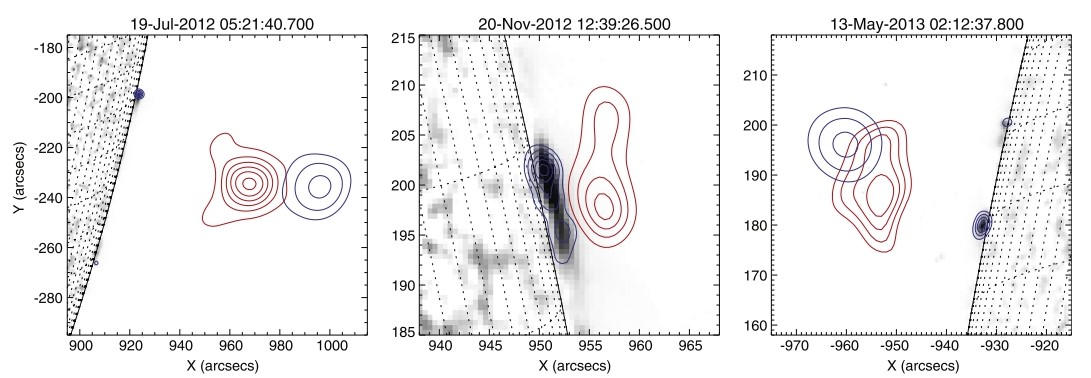
\includegraphics[width = \linewidth]{Figures/Krucker_2015_ApJ_802_19_page-0004.jpg}
    \caption{X-ray and optical imaging of the three flares at the peak time of the impulsive phase: the images are from HMI with the pre-flare image subtracted. The contours represent RHESSI Clean maps in the thermal (red, 12–15 keV) and non-thermal (blue, 30–80 keV) HXR range \citep{krucker15}.}
    \label{fig1}
\end{figure}

The spectral energy distribution of flares is one of the critical areas of interest in the physics of flares. A complete understanding of this will help us decode the physical processes involved in solar flares and help quantify their effects on solar spectral irradiance. Ideally, it would be essential to observe flares at all wavelengths simultaneously with sufficient spatiotemporal resolution to figure out the spectral energy distribution of flares. Unfortunately, this is generally not the case, and we have to rely on the sporadic observations made using ground-based instruments in the visible domain. As mentioned earlier, the majority of the flare energy is emitted in the NUV and visible domain. \cite{kretzschmar10,kretzschmar11}, performed statistical studies using a large number of flare observations across a wide energy range. They demonstrated, at the peak of the flare, about 70\% of the total energy was radiated in the continuum visible and NUV channel as illustrated in \ref{tab1}. SUIT would observe and resolve the solar flares within 200-400 nm using 8 NBs and 3 BBs. This, along with IRIS data, would help us comment on the energy distribution of flares of various classes.

%%--------------------------------------------%%
\begin{table}[]
    \centering
    \resizebox{\textwidth}{!}{%
    \begin{tabular}{||m{.1\linewidth}|m{.15\linewidth}|m{.17\linewidth}|m{.17\linewidth}|m{.17\linewidth}|m{.15\linewidth}||}
    \hline
    \hline
        Mean X-ray class & TSI(ergs) & Ratio $\frac{26-34nm}{TSI}$ & Ratio $\frac{0-50nm}{TSI}$ & Ratio $\frac{0.1-0.8nm}{TSI}$ & Ratio $\frac{continuum}{TSI}$\\
        \hline
        X3.2 & 5.9$\times~10^{31}$ & 0.9-0.8\% & 12-9\% & 1.2-1\% & 67\% \\
        M9.1 & 1.6$\times~10^{31}$ & 1.7-0.4\% & 23-5\% & 1-0.4\% & 85\% \\
        M4.2 & 1.3$\times~10^{31}$ & 2.2-0.5\% & 18-6\% & 0.6-0.3\% & 74\% \\
        M2.0 & 5.1$\times~10^{30}$ & 1.7-0.6\% & 18-6\% & 0.7-0.4\% & 69\% \\
        C8.7 & 3.6$\times~10^{30}$ & 1.5-0.5\% & 16-5\% & 0.4-0.2\% & 72\% \\
        \hline
    \end{tabular}}
    \caption{Spectral Energy Distribution from a sample of 2100 flares across various wavelengths\citep{kretzschmar11}.}
    \label{tab1}
\end{table}
%%--------------------------------------------%%

Finally, one of the major question of interest is how the Solar flares affect the Spectral Solar Irradiance (SSI) and Total Solar Irradiance (TSI) variability from a short to much longer, Solar Cycle timescale. \cite{kretzschmar10,kretzschmar11} performed statistical studies using a large number of flare observations across a wide energy range. For this purpose, they used the full Sun observations of Solar flux from Solar and Heliospheric Observatory (SoHO), three visible Solar irradiances from VIRGO/Solar Photometer (SPM) passbands centred on 402 nm, 500 nm, and 862 nm, respectively, from 1996 to 2008. Additionally, they also use the EUV irradiance in the ranges 0.1-50 nm and 26-34 nm measured by SOHO/Solar EUV Monitor \citep{judge98} and SXR measurements from GOES satellites. They showed that stacked TSI variation profiles during solar flares show variation at more than 2 sigma level during the peak flare time, indicating the presence of flare signals in the TSI measurements.

\begin{figure}[h!]
    \centering
    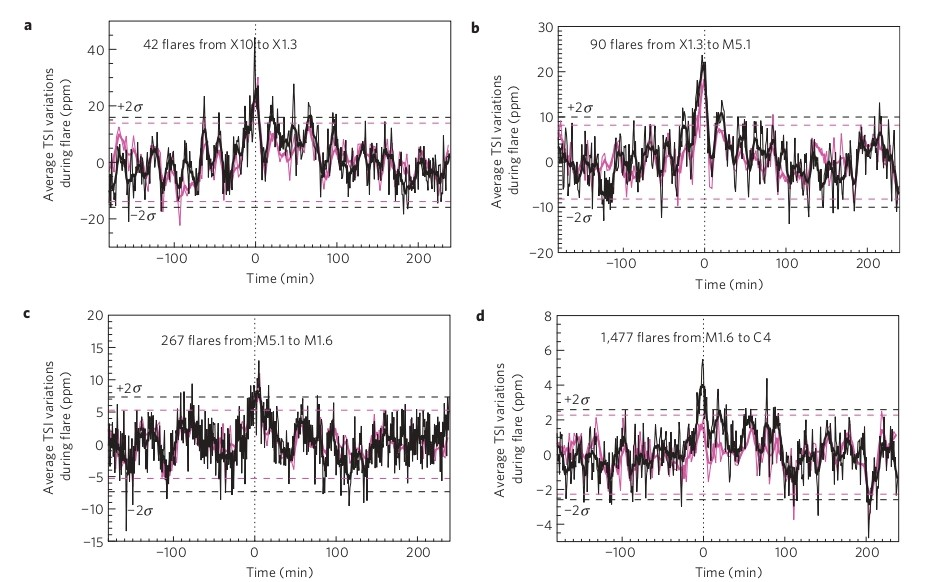
\includegraphics[width = \linewidth]{Figures/nphys1741_page-0002.jpg}
    \caption{Averaged TSI variations during flares. The TSI time-series averages over four exclusive sets of solar flares of decreasing amplitude. The black and pink curves correspond respectively to the TSI measured by the PMOV6 and the DIARAD radiometers. The dashed lines correspond to the 95\% confidence levels, while the vertical line denotes the peak time of the flare \citep{kretzschmar10}.}
    \label{fig2}
\end{figure}

This allows us to quantify the solar variability induced be solar flares of various timescales. With the help of SUIT, we would be able to localize the flare locations and study the change in SSI from the local environment in the 11 science filters. This information combined with TSI measurements can allow us to quantify the effect of flares of various energy scales on the TSI variability of the Sun. As, both the TSI and SSI variability directly or indirectly couples with various atmospheric parameters, we can also study the effect the flares have on them. For example, the Earth's atmospheric chemistry and composition respond to any changes in solar UV output in a very nonlinear fashion \citep{haigh07}. Since the number of flares also shows a change with solar activity, it is prudent to ask how much flares contribute to the solar spectral irradiance in NUV. This is particularly important because the irradiance in NUV plays a key role in heating the upper and middle layers of the Earth's atmosphere directly and their coupling with Stratosphere. It also directly influences the middle and lower atmosphere chemistry and composition via the Ozone-Oxygen cycle.


%%%%%%%%%%%%%%%%%%%%%%%%%%%%%%%%%%%%%%%%%%%%
\section{Throughput model and imaging performance of SUIT}\label{sec:suit_imaging}
%%%%%%%%%%%%%%%%%%%%%%%%%%%%%%%%%%%%%%%%%%%%

%%%%%%%%%%%%%%%%%%%%%%%%%%%%%%%%%%%%%%%%%%%%
\section{Filter Choice for SUIT}\label{sec:filter_choice}
%%%%%%%%%%%%%%%%%%%%%%%%%%%%%%%%%%%%%%%%%%%%

%%%%%%%%%%%%%%%%%%%%%%%%%%%%%%%%%%%%%%%%%%%%
\section{Photometric, Radiometric \& Spectral Calibration of SUIT}\label{sec:suit_cal}
%%%%%%%%%%%%%%%%%%%%%%%%%%%%%%%%%%%%%%%%%%%%

%NOTE THE LACK OF A BIBLIOGRAPHY CALL IN THIS FILE. BIBLIOGRAPHY WORK HAPPENS OUTSIDE THE CHAPTER TEX FILES.